\documentclass[conference]{IEEEtran}
\IEEEoverridecommandlockouts

\usepackage{cite}
\usepackage{amsmath,amssymb,amsfonts}
\usepackage{algorithmic}
\usepackage{algorithm}
\usepackage{graphicx}
\usepackage{textcomp}
\usepackage{xcolor}
\usepackage{soul}
\usepackage{subfig}
\usepackage{pifont}
\def\BibTeX{{\rm B\kern-.05em{\sc i\kern-.025em b}\kern-.08em
    T\kern-.1667em\lower.7ex\hbox{E}\kern-.125emX}}

\DeclareRobustCommand{\hlAdmin}[1]{{\sethlcolor{white}\hl{#1}}}% lime
\DeclareRobustCommand{\hlRevA}[1]{{\sethlcolor{white}\hl{#1}}}% yellow
\DeclareRobustCommand{\hlRevB}[1]{{\sethlcolor{white}\hl{#1}}}% pink
\DeclareRobustCommand{\hlRevC}[1]{{\sethlcolor{white}\hl{#1}}}% orange
\DeclareRobustCommand{\hlme}[1]{{\sethlcolor{white}\hl{#1}}}

\begin{document}

\title{CacheMigrate: Efficient Cache Migration for Load Balancing in Distributed Key-Value Storage Systems}

\author{
    \IEEEauthorblockN{
        Xianda Meng\IEEEauthorrefmark{1},
        Ammar Hawbani\IEEEauthorrefmark{1}\textsuperscript{*},
        Jiangyuan Chen\IEEEauthorrefmark{2},
        Abdulbary Naji\IEEEauthorrefmark{2},
        Liang Zhao\IEEEauthorrefmark{1}
    }
    \IEEEauthorblockA{\IEEEauthorrefmark{1}
        School of Computer Science,
        Shenyang Aerospace University,
        ShenYang, China \\
        Email: mengxianda1@stu.sau.edu.cn, anmande@ustc.edu.cn, lzhao@sau.edu.cn}
    \IEEEauthorblockA{\IEEEauthorrefmark{2}
        School of Computer Science and Technology,
        University of Science and Technology of China,
        Hefei, China \\
        Email: chenjy@mail.ustc.edu.cn, abdulbary@mail.ustc.edu.cn
    }
    \thanks{*Corresponding author: Ammar Hawbani (e-mail: anmande@ustc.edu.cn)}
}

\maketitle

\begin{abstract}
    Load imbalance in distributed key-value (KV) storage systems, especially under skewed access patterns across racks or clusters, can significantly degrade performance. We present CacheMigrate, a switch-assisted caching and migration framework that leverages programmable Top-of-Rack (ToR) switches for real-time hotspot detection, in-network caching, and per-key migration state tracking. By decoupling data movement from request handling, CacheMigrate minimizes service disruption and ensures strong consistency during live migration. A distributed migration state management design coordinates ToR and spine switches without centralized bottlenecks. We implement CacheMigrate on a P4-programmable switch and evaluate it using realistic workloads. Results show that CacheMigrate consistently delivers higher throughput and better load balance than existing approaches across diverse workload and system configurations.
\end{abstract}

\begin{IEEEkeywords}
    Key-value storage, load balancing, distributed systems, live migration, programmable switches
\end{IEEEkeywords}

\section{Introduction}

Large-scale key-value (KV) storage systems serve as the fundamental infrastructure for modern Internet services, including e-commerce and social networks. These systems are optimized for mission-critical operations that demand low-latency access, such as real-time data analytics, distributed machine learning training, and metadata indexing\cite{anwar2020customizable,wang2017metakv,8932384}. To address exponentially increasing I/O demands, geo-distributed multi-cluster architectures have become prevalent. Such architectures achieve scalability and fault tolerance through persistent data sharding \cite{decandia2007dynamo,nishtala2013scaling,10204945}. However, this design introduces a storage-specific challenge: cross-cluster load skew. Imbalanced access patterns during inter-cluster operations can create local hotspots. These hotspots degrade system throughput and cause tail latency spikes, potentially violating Service Level Objectives (SLOs)\cite{hong2013understanding, dean2013tail, 10758435,10830580}.

Caching is a fundamental method for load balancing in distributed systems. Theoretical analysis demonstrates that caching the top \(O (n \log n)\) hottest objects is sufficient to balance the load across $n$ storage nodes, with the cache size scaling only with the number of storage nodes, not the total object count\cite{fan2011small}. This principle is leveraged by NetCache\cite{jin2017netcache} to achieve intra-cluster load balancing via localized caching. However, when scaling to multiple clusters, caching within a single cluster becomes inadequate for addressing inter-cluster load imbalance. DistCache\cite{liu2019distcache} attempts to overcome this by merging caches from multiple clusters into a global cache. Despite this, its hotspot selection strategy leads to suboptimal cache utilization, as moderately popular objects in one cluster may receive more requests than the hottest objects in another cluster. This introduces consistency problems, as hotspots are replicated across clusters, complicating cache management. Therefore, static cache-based solutions like DistCache are insufficient for multi-cluster systems, where dynamic hotspot migration offers a more effective approach.

Current dynamic migration strategies for KV stores, including source\-based~\cite{kang2022remus} and destination-based~\cite{kulkarni2017rocksteady} migration, face significant performance challenges. Both aim to minimize downtime and ensure continuous query servicing, but each has limitations: source-based migration requires additional data transfers when requested data has not yet been copied to the destination, causing extra latency~\cite{kokkinos2016survey, lin2019mgcrab}; destination-based migration incurs round-trip delays to fetch unmigrated data. Hybrid approaches leverage both source and destination nodes to improve performance, but often add client-side tracking complexity and consistency-maintenance overhead~\cite{afonso2020combining}. Achieving efficient migration with minimal disruption remains a critical challenge.

\hlme{This paper introduces CacheMigrate, a novel solution addressing load-balancing challenges in multi-cluster storage systems.} By leveraging programmable switches, CacheMigrate integrates a high-speed in-network caching layer within the data plane. This approach enables several critical functionalities. Primarily, it serves as a real-time hotspot detector during migration initiation, identifying frequently accessed keys directly within the switch pipeline. Offloading this responsibility from the control plane allows CacheMigrate to trigger migrations swiftly and with minimal overhead, without burdening the source nodes.

A key feature of CacheMigrate is the decoupling of data movement from request servicing during migration. The system embeds per-key migration-state awareness directly into the data plane, enabling dynamic adjustments to the behavior of switches based on the progress of migration. For example, switches can reroute incoming requests or buffer updates as needed, ensuring that migration proceeds with minimal disruption to service and maintaining system correctness throughout the process.

To further enhance migration efficiency, CacheMigrate implements a distributed migration state management framework. This architecture assigns specific responsibilities to each component throughout the migration lifecycle. The source rack initiates migration by identifying and marking hot data, while the destination rack manages the finalization of migration. Spine switches play a crucial role by coordinating routing updates and ensuring that requests are consistently redirected. This distributed design offers scalable, fine-grained tracking of migration states on a per-key basis, effectively avoiding the performance bottlenecks commonly associated with centralized coordination.

In summary, we make the following contributions.
\begin{itemize}
    \item We propose CacheMigrate, a novel solution for dynamic load balancing in multi-cluster storage systems. By leveraging programmable switches, CacheMigrate integrates the data and control planes to enable real-time migration decisions and efficient resource coordination (\S\ref{subsec:system-architecture}).
    \item We design and implement a system that tightly couples in-network caching with distributed migration state management on emerging programmable switch hardware. This integration minimizes service disruption and ensures data consistency throughout the migration process (\S\ref{subsec:QueryHandling}).
    \item We build a working prototype using Barefoot Tofino switches and commodity servers integrated with TommyDS. Our evaluation shows that CacheMigrate achieves near-linear scalability with the number of racks, while incurring minimal overhead from its cache coherence protocol (\S\ref{sec:Experimental}).
\end{itemize}

To comprehensively detail CacheMigrate, we organize the paper as follows: Section \ref{sec_back_ground} reviews the background and motivation, Section \ref{sec:Design} presents the system design, Section \ref{sec:Experimental} reports experimental evaluation, Section \ref{sec:related_work} surveys related work, and Section \ref{sec:Conclusion} concludes with key findings and future directions.


\section{Background \& Motivation}
\label{sec_back_ground}

\subsection{Caching \& Migration Strategies}

Caching is a fundamental technique for load balancing in distributed storage systems. It improves latency and reduces backend load by storing the most frequently accessed keys. Prior work shows that caching the top \(O (n \log n)\) hottest items across $n$ nodes is enough for near-optimal balance, regardless of dataset size~\cite{fan2011small}. This works because real workloads are highly skewed, with a small fraction of data serving most requests~\cite{atikoglu2012workload}. Systems like NetCache~\cite{jin2017netcache} use localized caching and compact metadata to balance intra-cluster loads, scaling with cluster size rather than dataset cardinality. Caching only a few thousand objects can balance hundreds of nodes, even under skewed workloads such as Zipfian-0.9 and Zipfian-0.99.

However, static caching has limitations in multi-cluster systems. Global-local popularity divergence occurs when moderately popular items in busy clusters create more load than globally popular items elsewhere. Cache efficiency also drops when per-cluster caches are merged into a global hierarchy, lowering hit rates by over 25\%~\cite{medeiros2020survey}. Static caching must therefore evolve into dynamic, adaptive mechanisms.

In distributed KV stores, dynamic re-sharding helps balance load, improve locality, and scale as clusters grow. Live migration moves data without interrupting requests, mitigating hot spots~\cite{kulkarni2017rocksteady, katsarakis2021zeus}. Source-based migration serves requests from the source while incrementally copying data; destination-based migration lets the destination fetch data on demand. Both maintain availability but trade off latency: source-based delays replication, destination-based suffers round-trip fetches. Hybrid strategies~\cite{vasilakis2020hybrid2, young2019tictoc} combine the two, but require real-time metadata for ownership tracking, adding overhead and complexity. These issues intensify in multi-cluster environments. Workloads can shift across regions, requiring rapid data reallocation~\cite{decandia2007dynamo}. Centralized migration control becomes a bottleneck, slowing adaptation to changing demand.

\subsection{Load Balancing in Multi-cluster Storage}
Multi-cluster load balancing is becoming increasingly crucial as modern distributed storage systems extend across geographically dispersed clusters serving diverse user populations~\cite{bachar2023optimizing, duraisamy2023towards}. In such environments, request patterns are highly variable and can change unpredictably~\cite{shen2010request}. A moderately popular key in one cluster may generate more load than the globally hottest key in another, leading to significant cross-cluster imbalances if static policies are maintained. Traditional solutions, like static in-cluster caching and periodic rebalancing, fail to effectively address these dynamics, resulting in degraded performance and increased tail latency.

To overcome these issues, dynamic strategies are needed that can adapt to workload changes in real time without incurring excessive coordination overhead. To this end, we propose distributed migration state management as a key design principle underlying our work. \hlme{By decentralizing migration control, CacheMigrate allows each cluster to independently monitor progress, trigger state transitions, and coordinate updates via programmable switches in the data plane, thereby achieving faster and more efficient load balancing.} This decentralized approach allows the system to dynamically redistribute hot data, reducing reliance on control-plane interventions and significantly improving responsiveness and efficiency for cross-cluster load balancing.


\section{CacheMigrate Design}
\label{sec:Design}

\begin{figure}[!t]
    \centering
    \subfloat[Per Cluster Architecture.]{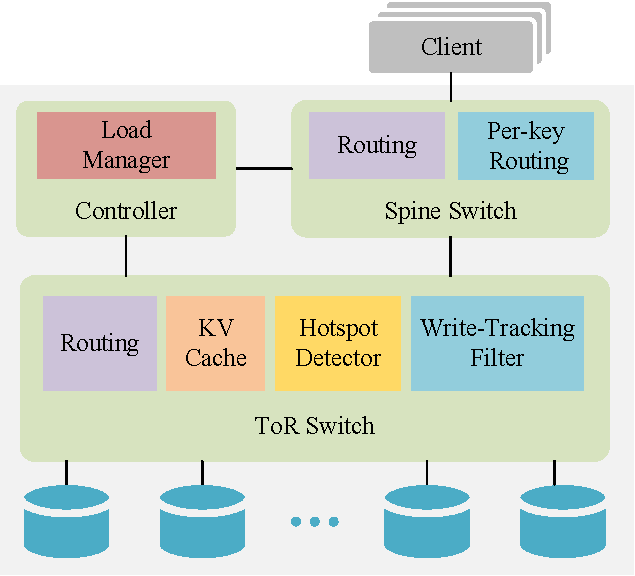
\includegraphics[width=0.8\linewidth]{figures/per-cluster_architecture.pdf}
        \label{fig:architecture}}\\
    \subfloat[CacheMigrate Network Protocol.]{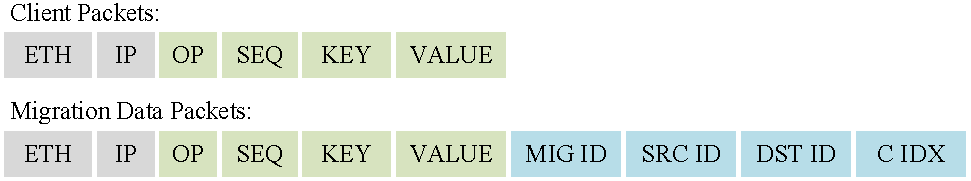
\includegraphics[width=0.8\linewidth]{figures/Protocol.pdf}
        \label{fig:Protocol}}
    \caption{System Architecture.}
\end{figure}

\subsection{System Architecture}
\label{subsec:system-architecture}

Fig~\ref{fig:architecture} shows the per-cluster architecture of CacheMigrate. Each Top-of-Rack (ToR) switch has in-network caching, real-time hotspot detection, and per-key migration state tracking. This design allows dynamic coordination through spine-level routing and control-plane orchestration. CacheMigrate is implemented as an IP-based L3 protocol, and its packet format is illustrated in Fig~\ref{fig:Protocol}.

\paragraph{ToR switch}
The ToR switch handles three core functions to support seamless migration:
(1) It maintains a KV cache to serve client requests quickly and hide migration delays;
(2) It includes a hotspot detector that identifies frequently accessed keys in real time, enabling fast migration when triggered;
(3) It implements a Write-Tracking filter to track updates during migration and ensure write consistency.
Together, these functions make the ToR switch essential for efficient, transparent migration in CacheMigrate.

\paragraph{Spine switch}
The spine switch updates routing entries once migration completes, ensuring that client requests are forwarded to the correct destination servers. It maintains global routing consistency across the network and supports load balancing by evenly distributing requests across clusters. By dynamically adapting to migration status, it ensures efficient and reliable request routing.

\paragraph{Controller}
The controller, or Load Manager, monitors system-wide load metrics from all ToR switches. It detects imbalances and triggers migrations to redistribute load. Based on real-time statistics, it selects source racks and issues migration commands. Its global view and dynamic decision-making allow CacheMigrate to scale effectively under varying workloads.

\paragraph{Servers \& clients}
Storage servers store KV data and transfer selected keys during migration under ToR switch control, without handling hotspot detection or key selection. Destination servers validate data and signal completion. Clients use the CacheMigrate library to send commands and infer migration status by comparing response sources with original destinations, without explicit coordination.

In our design, each system layer is assigned responsibilities based on its capabilities. The control plane makes load balancing decisions and initiates migrations. The source cluster selects migration content and triggers the process, while the destination cluster ensures data consistency and commits state transitions. Spine switches handle dynamic routing updates, ensuring accurate redirection of client requests throughout migration. This division of responsibilities enables efficient, consistent, and low-overhead migration without relying on centralized orchestration for every step.

\subsection{Challenges and Goals}

\subsubsection{Decentralizing migration control}
In large-scale systems, centralized tracking of migration progress becomes a bottleneck. The control plane must maintain per-key migration state across thousands of storage nodes, which limits scalability and responsiveness. Moreover, programmable switches have limited on-chip resources, making it impractical to store large volumes of state directly in the data plane.

To address this, CacheMigrate adopts a decentralized approach to migration control. Instead of relying on a central controller, each cluster manages per-key migration state locally. The source and destination coordinate with their ToR switches to track progress and update status. Routing updates are handled by spine switches based on key states, allowing the system to support concurrent migrations without overloading the control plane. This design reduces coordination overhead and enables scalable, fine-grained migration with minimal switch resource usage.

\subsubsection{Service disruption during migration}
A key challenge in live migration is avoiding service disruption when a key is in transit. During this period, client requests may arrive at either the source or destination cluster, risking increased latency, incorrect routing, or request failure. Existing systems often require coordination between endpoints or rely on clients to retry failed requests, resulting in inconsistent performance.

CacheMigrate addresses this challenge by leveraging in-switch caching to isolate client request handling from the underlying migration process. Specifically, the ToR switch continues to serve queries from its cache even as the backend migrates data between clusters. This allows client requests to be processed without delay, regardless of whether the migration has completed. \hlme{The switch updates its routing only after the destination confirms the migration is complete.} As a result, migration can proceed in the background without interrupting service, enabling seamless and transparent request handling throughout the migration lifecycle.

\subsubsection{Data consistency}
Maintaining consistency during migration is challenging when reads and writes continue.
Conventional systems risk violations if updates hit both source and destination, or if stale data is served due to delayed synchronization.
These risks grow in distributed settings with higher latency and coordination costs.

CacheMigrate adds complexity by serving queries from in-switch caches during migration.
While this avoids service disruption, it risks stale reads and conflicting writes if cached data diverges from the backend.

To address this, CacheMigrate tracks migration state per key and enforces strict state transitions.
Writes are redirected to the correct backend according to the migration phase.
Switches permit cache reads only for consistent keys, and invalidate entries on state changes.
This prevents duplicate writes and stale responses, ensuring strong consistency throughout migration.

\subsection{Overview of Migration Workflow}

\begin{figure}[!t]
    \centering
    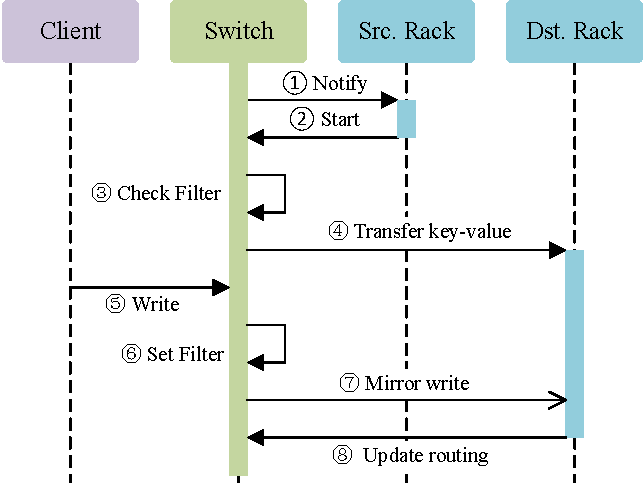
\includegraphics[width=0.8\linewidth]{figures/migration_flow.pdf}
    \caption{Migration Flow.}
    \label{fig:migration_flow}
\end{figure}

In the previous sections, we have outlined the roles of key components involved in the CacheMigrate system, including the storage servers, clients, and control plane. These components work together to facilitate seamless data migration. To provide a clearer understanding of how these components interact during the migration process, we now present an overview of the migration workflow.

Fig~\ref{fig:migration_flow} illustrates the basic KV migration process in CacheMigrate. \hlme{Most migration tasks are handled by the destination rack to minimize load on the source rack.} When the control plane detects that a rack is overloaded, it triggers a migration request (Step~\ding{172}). The source rack then informs its ToR switch to initiate the migration. \hlme{The source server does not select migration content, further reducing its workload} (Step~\ding{173}).

The ToR switch in the source rack selects the keys to migrate and prepares to send them to the destination rack (Step~\ding{175}). Before sending, it checks an internal Write-Tracking filter to decide whether a key is eligible for migration (Step~\ding{174}). Once the destination rack receives the keys, it updates the routing table via the switch to ensure future requests are directed to the new location (Step~\ding{179}).

Importantly, clients are unaware of the migration. During the process, if a write request targets a key being migrated (Step~\ding{176}), the Write-Tracking filter logs it to prevent further migration of that key (Step~\ding{177}). The switch also mirrors the write request to the destination rack (Step~\ding{178}). After receiving the mirrored request, the destination rack completes the migration and takes over ownership of the data (Step~\ding{179}).


\subsection{Migration State Management}

\subsubsection{Load manager}
\label{subsec:load_manager}
The Load Manager is responsible for continuously monitoring cluster-level load and initiating migration procedures when necessary. Specifically, it periodically collects per-port counters from each ToR switch to estimate metrics such as request rates, cache hit ratios, and heavy-hitter statistics. Based on these aggregated measurements, it computes a load index for each rack and determines whether sustained overload conditions are present.

Global cache hit rate is a key indicator of the system's capacity to absorb request load without resorting to migration. For each time interval \( t \), we define the global cache hit count \( H(t) \) as
\begin{equation}
    H(t) = \sum_{i = 1}^{N} \mathrm{Hits}_i(t).
\end{equation}
The per-second cache hit rate is given by
\begin{equation}
    \mathrm{HitRate}(t) = \frac{H(t)}{\sum_{i = 1}^{N} \mathrm{TotalRequests}_i(t)}.
\end{equation}
When the global hit rate remains high, the majority of requests are satisfied directly by ToR caches, reducing backend load and diminishing the urgency of migration. Conversely, sustained decreases in global hit rate signal that cache resources are insufficient to accommodate shifting access patterns, thereby increasing the risk of server overload. CacheMigrate monitors global hit rate trends over time and dynamically adjusts migration policies accordingly. In particular, lower hit rates trigger more aggressive migration, both in terms of the frequency of migration events and the volume of keys selected for transfer. This adaptive strategy ensures that migration bandwidth is allocated where it can most effectively alleviate load imbalance.

The load index $L$ is defined as
\begin{equation}
    \label{eq:load_index}
    L = \alpha \cdot \frac{b(t) + p(t)}{\Delta t} + \beta \cdot \mathrm{AverageTrend},
\end{equation}
where $\alpha$ and $\beta$ are configurable weighting factors (e.g., $\alpha$ = 0.9, $\beta$ = 0.1), \( b(t) \) and \( p(t) \) denote bytes and packets observed in the most recent interval,
and \( \mathrm{AverageTrend} \) measures the mean incremental rate of change across recent intervals. This formulation allows the system to capture both instantaneous overload and sustained trends when making migration decisions.

When the load index exceeds a configurable threshold, the Load Manager notifies the source rack to initiate migration. Importantly, it does not participate in selecting which keys to migrate; this decision is delegated entirely to the source rack, which relies on its local heavy-hitter detection and cache metadata to identify suitable migration candidates. This design decouples global load monitoring from per-rack migration planning, reducing the complexity of the control plane and improving scalability.

\subsubsection{Write-Tracking filter}
\label{subsec:write_tracking}
we use a probabilistic Bloom filter (BF) on each ToR switch to track keys modified during migration. This compact structure stores millions of entries with only a few hundred kilobytes, avoiding the high memory cost of explicit per-key state. When a write occurs after migration starts, the key is inserted into the filter; during migration, a match causes the system to skip transferring that key to prevent stale data propagation, while still mirroring and routing writes for correctness (\S\ref{subsec:QueryHandling}). Although BF have a false positive probability \( p \approx \left(1 - e^{-\frac{k n}{m}}\right)^k \), we treat matches conservatively to ensure correctness. Our P4-based implementation allocates \( 2^{20} \) bits and three hash functions, yielding a false positive rate below 1\% in typical workloads, with all operations running at line rate without control-plane involvement.
 
\subsubsection{Distributed state management}
Centralized coordination is often a scalability bottleneck in distributed systems. Maintaining per-key migration progress globally imposes high coordination overhead and increases latency, especially under dynamic or concurrent migrations. To address this, CacheMigrate adopts a distributed approach, assigning migration responsibilities to different components based on their roles and visibility.

The control plane, which has a global view of cluster-wide load conditions, is responsible for initiating migrations (\S\ref{subsec:load_manager}). The source cluster triggers the migration process, since it owns the initial state and can identify candidate data. To assist this process, the source ToR switch employs a Write-Tracking filter to monitor write activity and mark hot keys for migration (\S\ref{subsec:write_tracking}). This ensures that frequently updated data is prioritized and captured accurately. The destination cluster, in turn, completes the migration by validating data consistency and signaling readiness to serve future requests—marking the natural end of the migration.

Finally, routing updates are handled by spine switches. As backbone nodes that interconnect all clusters, spine switches are ideally positioned to perform consistent path redirection across the system. Once a migration completes, spine switches update their forwarding logic to route subsequent client requests to the new data location. This division of responsibilities enables scalable, fine-grained coordination without relying on global synchronization.


\subsection{Query Handling During Migration}
\label{subsec:QueryHandling}

\begin{figure}[!t]
    \renewcommand{\algorithmicrequire}{\textbf{Input:}}
    \renewcommand{\algorithmicensure}{\textbf{Output:}}
    \begin{algorithm}[H]
        \caption{Query Handling During Migration}
        \label{alg:query_handling}
        \begin{algorithmic}[1]
            \REQUIRE Request \texttt{req}, Key-Value cache \texttt{cache},  \\Write-Tracking filter \texttt{filter}
            \ENSURE Correct routing and consistency during migration

            \IF{\texttt{req.key} exists in \texttt{cache} and is valid}
            \IF{\texttt{req.op == GET}}
            \STATE \texttt{req.value} $\leftarrow$ \texttt{cache[req.key]}
            \RETURN \texttt{req}
            \ELSIF{\texttt{req.op == SET}}
            \STATE \texttt{cache[req.key].valid} $\leftarrow$ \texttt{false}
            \STATE \texttt{routing(req, source)}
            \STATE \texttt{mirror(req, destination)}
            \STATE \texttt{filter.set(req.key)}
            \ENDIF
            \ENDIF
        \end{algorithmic}
    \end{algorithm}
\end{figure}

When a key is selected for migration, there is a transition period from the moment the source rack initiates migration until the spine layer updates its routing table to forward future requests to the new server. During this period, CacheMigrate uses the cache layer on the ToR switch to serve all related queries. This ensures that clients experience no visible disruption or downtime. Algorithm~\ref{alg:query_handling} shows the pseudocode for query handling during migration.

\paragraph{Read requests}
When a client sends a read request for a migrating key, the system first checks the ToR cache. If the key is found in the cache, the switch replies directly. This avoids backend involvement and reduces latency. If the key is not in the cache, the request is sent to the source server. The source server remains responsible for the key until migration finishes. After migration completes and the routing is updated, new read requests go to the destination server (Algorithm~\ref{alg:query_handling}, lines 2-4). This mechanism ensures uninterrupted read service and isolates the client from migration details.

\paragraph{Write requests}
Write operations on keys under migration require consistency protection. Before the routing is updated at the spine switches, the system always uses the source rack as the authoritative replica. When a write request arrives, the data plane performs two actions. It forwards the request to the source server, which processes and acknowledges the write. \hlme{Simultaneously, it mirrors the request to the destination server to maintain data consistency.} The key is also added to the Write-Tracking Filter. This filter tracks keys that are modified during migration. During the transfer phase, the migration engine checks the filter. If the key is marked, the system skips migrating it to avoid overwriting newer data (Algorithm~\ref{alg:query_handling}, line 5-9). This conservative approach ensures that no stale data reaches the destination, even when writes occur during migration.


\subsection{Cache Consistency During Migration}

During key migration, ensuring cache consistency is critical to maintaining correct system behavior. Clients may issue read or write requests to a key while it is being moved between racks. If these operations are not properly coordinated, they can lead to consistency violations. In particular, we focus on two common scenarios: Read-After-Write (RAW) and Write-After-Write (WAW) conflicts. These conflicts must be carefully handled to prevent stale reads or inconsistent writes.

\paragraph{RAW}
A client may issue a write followed immediately by a read to the same key. Since all writes are forwarded to the source server and mirrored to the destination, the source remains the authoritative node until the migration completes. To ensure the latest value is returned, all reads during migration are routed to the source server, even if the destination has already received mirrored updates.

\paragraph{WAW}
\hlme{For this scenario, a client performs multiple writes to the same key during an ongoing migration.} CacheMigrate preserves write ordering at the source, which serializes and acknowledges all writes as the primary replica. Mirrored writes are sent to the destination in the same order. Additionally, the Write-Tracking filter ensures that no stale state from the source is copied over after these writes, preserving the correct final state at the destination.


\section{Experiments \& Evaluation}
\label{sec:Experimental}

\subsection{Experimental Setup}

We have implemented a full-stack prototype of CacheMigrate to evaluate its feasibility and performance. The system consists of cache-enabled programmable switches, a centralized controller, and a set of storage servers and clients.

Our experiments are conducted on a dedicated cluster of commodity servers connected via a high-speed data center network. Each server is equipped with an Intel Xeon Silver 4310 CPU (12 cores @ 2.10\,GHz), 128\,GB DDR4 memory, and a Mellanox ConnectX-5 NIC (100\,Gbps) with DPDK~\cite{dpdkDPDKx2013} enabled for kernel-bypass packet processing. The network fabric includes Mellanox SN2700 (100\,GbE) switches and one Barefoot Tofino~\cite{tofino} programmable switch with a switching capacity of 6.5\,Tbps. All servers run \texttt{Ubuntu~20.04} with \texttt{Linux kernel~5.15}.

To maximize testbed utilization, we partition both the programmable switch and servers into multiple logical components, running real switch data-plane programs and server software simultaneously. Specifically, the Barefoot Tofino switch is configured to emulate 32 spine switches, 32 leaf switches, and 32 client-access switches, while the servers act as storage nodes, controller instances, and clients in parallel. Each switch cache stores 128 KV pairs by default, with both keys and values being 128-bit in size.

We deploy \texttt{TommyDS}~\cite{githubGitHubAmadvancetommyds} as the backend KV store, configuring each physical server to emulate 32 racks, with each rack hosting 32 server instances. This setup allows the testbed to scale to a large number of logical servers while using only a limited number of physical machines, ensuring realistic request handling and migration behavior under high concurrency. \hlme{We also rate-limit \texttt{TommyDS} to prevent individual servers from becoming bottlenecks and to emulate realistic aggregate throughput.}

Workloads are generated using the Yahoo! Cloud Serving Benchmark (YCSB)~\cite{cooper2010benchmarking} with different hotspot intensities, characterized by Zipfian distribution parameters ($\theta = 0.9$, $0.95$, and $0.99$). These workloads allow us to evaluate system performance under varying degrees of load skew.

\subsection{Baselines}

We compare CacheMigrate against three representative approaches:
\textbf{DistCache}~\cite{liu2019distcache}, a hierarchical caching framework that partitions cache space across multiple layers to balance load and reduce backend traffic.
\textbf{NetCache}~\cite{jin2017netcache}, a switch-based in-network caching system that uses programmable switches to store hot objects and directly serve client requests, thereby reducing load on backend servers.
\textbf{NoCache}, a baseline without any caching, where all requests are sent directly to backend servers, serving as the lower bound for performance.


\subsection{Results \& Analysis}

\begin{figure*}[!t]
    \centering
    \subfloat[Throughput With Different Skewness.]{
        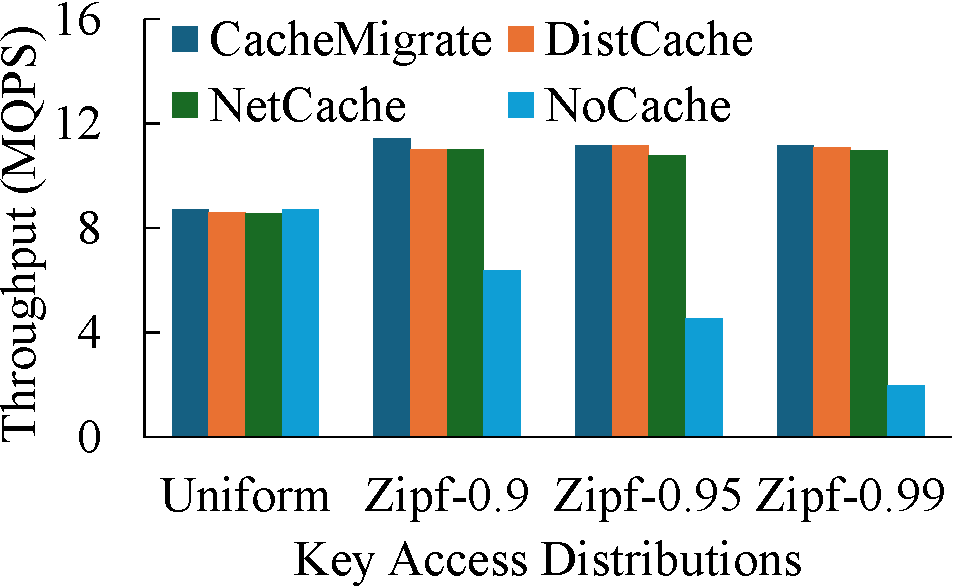
\includegraphics[width=0.3\linewidth]{figures/Throughput_with_different_skewness.pdf}
        \label{fig:Throughput_with_different_skewness}
    }
    \hfill
    \subfloat[Latency]{
        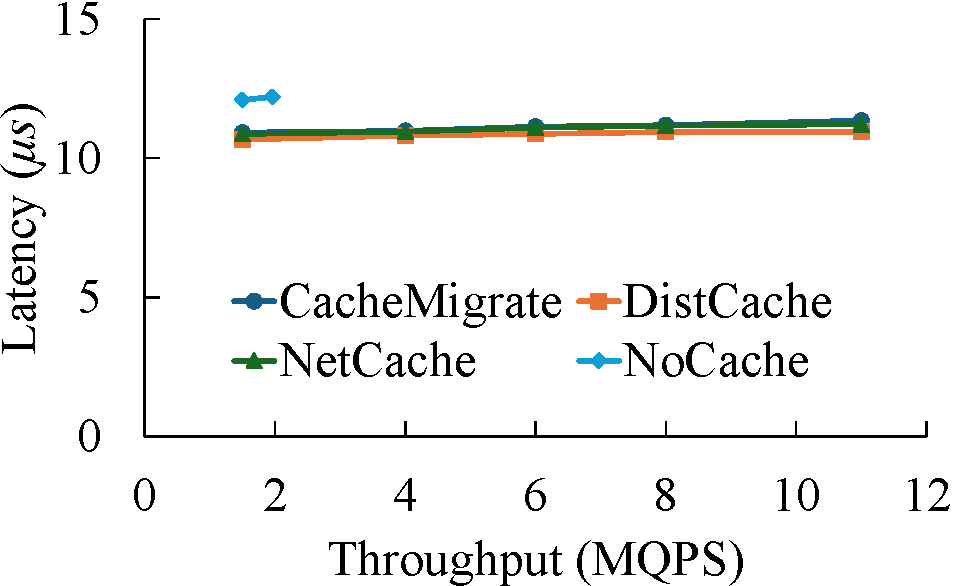
\includegraphics[width=0.3\linewidth]{figures/Latency.pdf}
        \label{fig:Latency}
    }
    \hfill
    \subfloat[Imbalance]{
        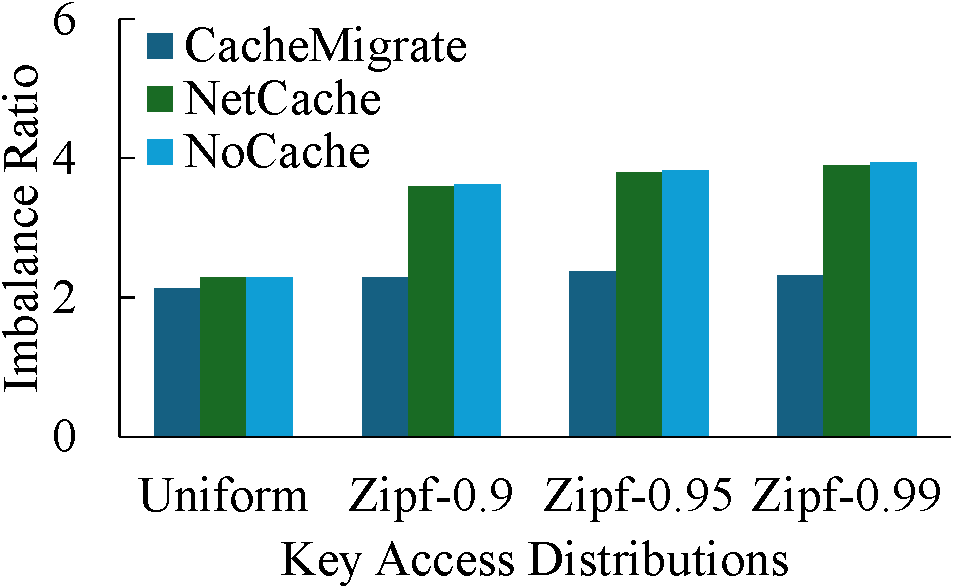
\includegraphics[width=0.3\linewidth]{figures/Imbalance.pdf}
        \label{fig:Imbalance}
    }
    \hfill
    \subfloat[Impact of Cache Size.]{
        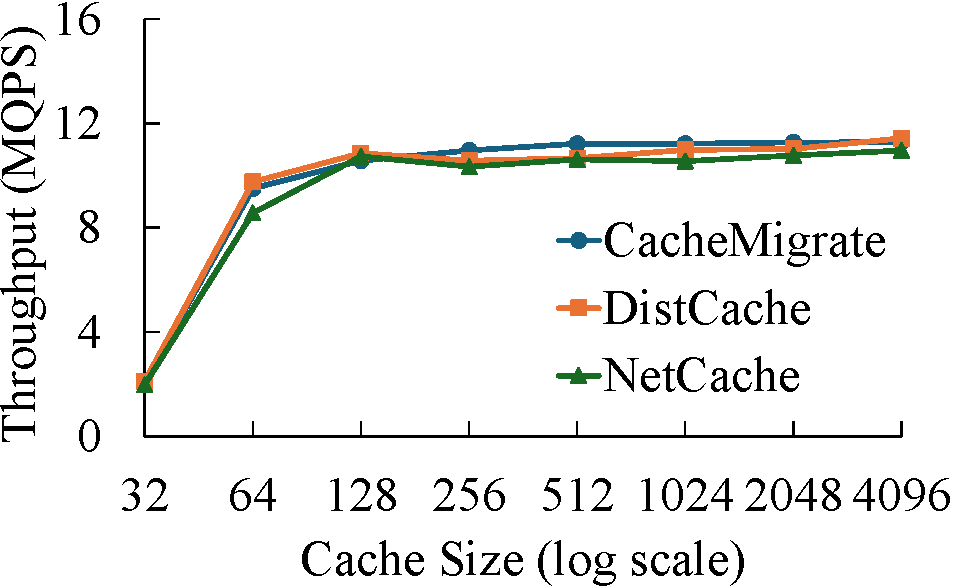
\includegraphics[width=0.3\linewidth]{figures/Impact_of_cache_size.pdf}
        \label{fig:Impact_of_cache_size}
    }
    \hfill
    \subfloat[Impact of Write Ratio.]{
        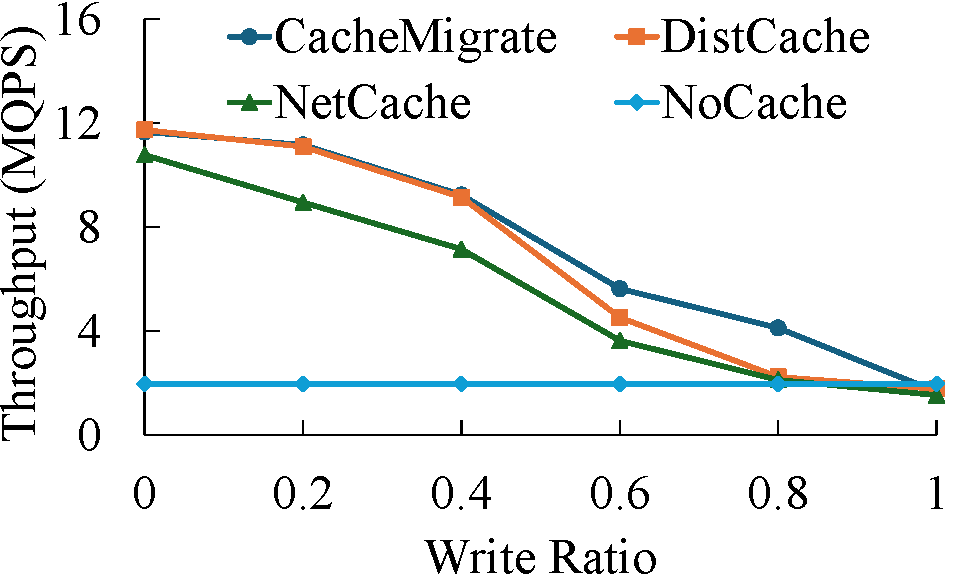
\includegraphics[width=0.3\linewidth]{figures/Impact_of_write_ratio.pdf}
        \label{fig:Impact_of_write_ratio}
    }
    \hfill
    \subfloat[Scalability]{
        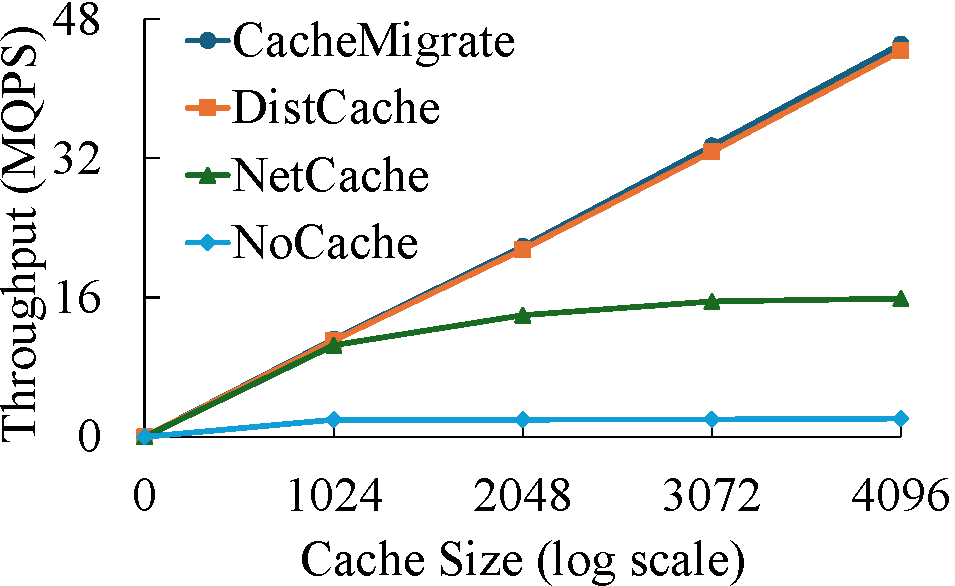
\includegraphics[width=0.3\linewidth]{figures/Scalability.pdf}
        \label{fig:Scalability}
    }

    \caption{System Performance.}
    \label{fig:System_Performance}
\end{figure*}

\subsubsection{Throughput with different key access distributions}
Fig~\ref{fig:Throughput_with_different_skewness} compares the throughput of the four approaches under varying load skewness. CacheMigrate maintains higher throughput by dynamically redistributing key placements to adapt to different skew levels. As inter-rack load skew increases, NetCache suffers from rack-level imbalance, leading to a slight throughput drop. DistCache achieves higher throughput by caching a larger set of objects, partially mitigating the impact of skew.


\subsubsection{Latency}
\hlRevA{As shown in} Fig.~\ref{fig:Latency}, \hlRevA{across the throughput range of 1.5 to 11 MQPS, CacheMigrate maintains a low P99 latency, comparable to NetCache and DistCache. In contrast, NoCache exhibits significantly higher latency and reaches saturation at 2 MQPS. This indicates that CacheMigrate effectively mitigates latency spikes under increasing load by leveraging cache migration, whereas the absence of caching leads to early saturation and degraded tail performance.}

\subsubsection{Imbalance}
\hlRevC{Using} Equation~\eqref{eq:load_index}, \hlRevC{we compute each rack's load index and define the Imbalance Ratio as the maximum load divided by the average. As shown in} Fig.~\ref{fig:Imbalance}, \hlRevC{CacheMigrate consistently achieves the lowest imbalance: 2.13 under uniform traffic and 2.31 under highly skewed Zipf-0.99 workloads, whereas NetCache and NoCache reach 3.9. This demonstrates that CacheMigrate effectively balances load across racks, even under highly skewed access patterns.}

\subsubsection{Impact of cache size}
Fig.~\ref{fig:Impact_of_cache_size} shows the throughput of the three mechanisms under different switch cache sizes. Larger caches absorb more hotspot requests, reducing backend load. CacheMigrate further enhances cache utilization by dynamically reallocating keys during migration, making full use of additional capacity to balance load across racks.

\subsubsection{Impact of writ ratio}
As shown in Fig.~\ref{fig:Impact_of_write_ratio}, the system throughput decreases gradually as the write ratio increases. This trend is consistent across all compared mechanisms, with CacheMigrate maintaining a performance advantage due to its ability to effectively handle write-induced cache invalidations.

\subsubsection{Scalability}
Fig.~\ref{fig:Scalability} \hlRevC{shows the scalability of the different caching schemes as the number of cached hot objects increases. CacheMigrate and DistCache scale nearly linearly, demonstrating effective utilization of additional cache capacity. In contrast, NetCache grows sublinearly and NoCache shows minimal improvement. These results highlight that CacheMigrate can efficiently leverage larger cache sizes to sustain high throughput under increasing workloads.}


\subsubsection{Impact of migrateion size}
\begin{figure}[!t]
    \centering
    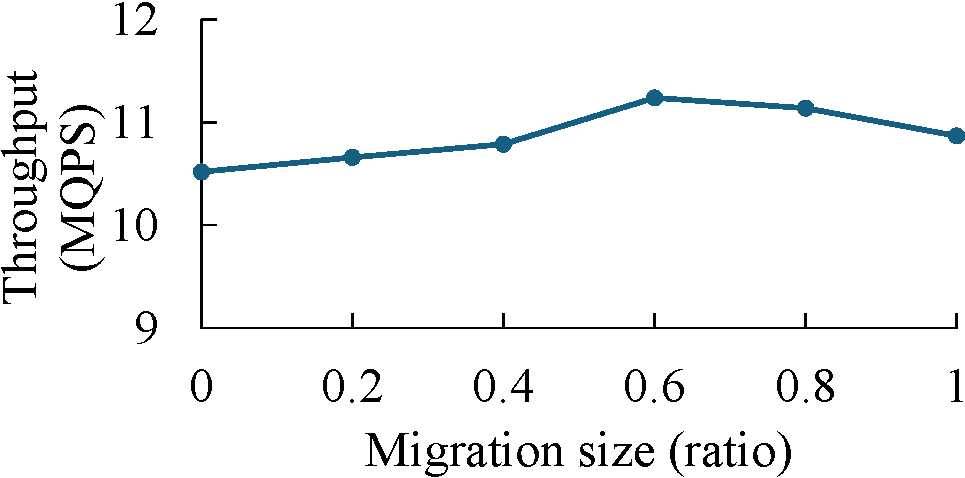
\includegraphics[width=0.7\linewidth]{figures/Impact_of_migrateion_size.pdf}
    \caption{Impact of Migration Size}
    \label{fig:Impact_of_migrateion_size}
\end{figure}

\hlAdmin{We evaluate the impact of migration size on system throughput by varying the ratio of migrated data to the total switch cache capacity from 0 to 1. As shown in} Fig.~\ref{fig:Impact_of_migrateion_size}, \hlAdmin{throughput increases with moderate migration (up to about 0.6 ratio) as load becomes more balanced, but declines when the ratio exceeds 0.6 due to higher migration overhead. This result indicates an optimal migration size that balances load redistribution and migration cost.}

\subsubsection{Hardware resources}
\begin{table}[htbp]
    \caption{Hardware Resource Usage Summary}
    \begin{center}
        \begin{tabular}{cccc}
            \hline
            \textbf{SRAMs} & \textbf{TCAMs} & \textbf{Map RAMs} & \textbf{Logical Tables} \\
            \hline
            124            & 13             & 50                & 65                      \\
            \hline
        \end{tabular}
        \label{tab:resource_summary}
    \end{center}
\end{table}

As shown in Table~\ref{tab:resource_summary}, the hardware resources encompass memory blocks, lookup tables, and logic units required to implement the data plane pipeline. These resources determine the design's capacity, flexibility, and performance characteristics across different processing stages.

\subsubsection{Protocol efficiency}

To evaluate CacheMigrate, we first consider the Ethernet/IPv4 overhead, which consists of 14 bytes for the Ethernet header and 20 bytes for the IPv4 header. The CacheMigrate-specific headers are 42 bytes for \texttt{Client Packet} and 52 bytes for \texttt{Migration Data Packet}(Fig~\ref{fig:Protocol}).

For a \texttt{Client Packet} carrying 42 bytes of payload, the total packet length is 76 bytes, yielding a protocol efficiency of $\eta_{KV} \approx 55.3\%$. For a \texttt{Migration Data Packet} carrying 52 bytes of payload, the total packet length is 86 bytes, giving an efficiency of $\eta_{Migrate} \approx 60.5\%$.

By packing multiple control fields into a compact header, CacheMigrate reduces protocol overhead and achieves high throughput for rack-level key migration.


\section{Related Work}
\label{sec:related_work}

\textbf{Cache systems.}
Memcached~\cite{memcachedMemcachedDistributed} and Redis~\cite{redisRedisRealtime} Cluster improve performance for read-heavy workloads but face challenges in write-heavy scenarios and in maintaining consistency across distributed deployments~\cite{ghemawat2003google, beaver2010finding}. These limitations motivate more advanced cache management and migration strategies to balance load and optimize data locality.

\textbf{Cache migration mechanisms.}
Cache migration moves data between nodes to improve hit rates and balance load, but often incurs overhead that can reduce throughput. Prior work focuses on hot-object migration or consistency maintenance. CacheMigrate builds on these ideas with more efficient, low-overhead migration.

\textbf{Programmable data plane.}
Programmable data planes such as P4~\cite{opennetworkingOpenNetworking} and Barefoot Tofino~\cite{tofino} enable custom, fine-grained load balancing directly in the network. This approach optimizes traffic distribution and reduces congestion. CacheMigrate leverages these capabilities to enhance cache migration and request forwarding efficiency.


\section{Conclusion}
\label{sec:Conclusion}

We present CacheMigrate, a switch-assisted caching and migration framework that dynamically adapts to workload skewness in distributed KV stores. \hlme{Leveraging programmable switches for hot-object caching and fine-grained migration control, CacheMigrate improves throughput and load balance across diverse workloads.} Our evaluation shows that in-network coordination effectively mitigates rack-level imbalances while maintaining strong consistency. Looking ahead, we plan to offload more coordination and state management into the switch data plane to reduce control-plane overhead and enable faster, fully in-network adaptation to workload dynamics. \hlRevB{In addition, we will investigate the integration of security mechanisms and enhanced fault-tolerance strategies to ensure reliable operation under node or switch failures and maintain data integrity during migration.} \hlRevA{Furthermore, we plan to evaluate the energy consumption and power overhead introduced by migration operations, additional packet processing, and Bloom Filter queries to provide a more comprehensive assessment of system efficiency.}



\section*{Acknowledgment}

\vspace*{-0.5 \baselineskip} This paper was supported by Shenyang Aerospace University Talent Research Start-up Fund under Grant 502/120423005.  LLM was used for proofreading.

\bibliographystyle{IEEEtran}
\bibliography{references}

\end{document}
